\chapter{Revisão da Literatura}

Será apresentado neste capítulo o conjunto de trabalhos acadêmicos relevantes para o tema desta pesquisa, bem como a metodologia utilizada para definí-lo.

\section{Artigos científicos}

\subsection{Método de pesquisa}

O processo de pesquisa utilizado neste projeto foi baseado no método chamado revisão sistemática. Segundo Barbara Kitchenham \cite{Barbara04}, uma revisão sistemática da literatura consiste em identificar, avaliar e interpretar todas pesquisas disponíveis relevantes a uma determinada questão, tópico ou área de interesse. Este tipo de pesquisa requer a definição de alguns pontos:

\begin{itemize}
	\item A(s) questão(ões) a ser(em) respondida(s) ao final da pesquisa
	\item A estratégia utilizada (fontes consultadas, termos buscados, etc.)
	\item Critérios de seleção e exclusão de material
\end{itemize}

A necessidade da adoção de uma revisão sistemática decorre da exigência de se sumarizar todo um conjunto de informações existentes no que tange à adoção de metodologias ágeis por parte de empresas de desenvolvimento de software. A partir deste estudo, pôde-se criar um arcabouço para a elaboração dos questionários que foram utilizados neste projeto. A Figura \ref{fig:metodologia} mostra uma visão alto nível da metodologia adotada para encontrar trabalhos acadêmicos que possuem tais informações.

\begin{figure}[H]
	\centering
	\captionsetup{justification=centering,margin=2cm}
	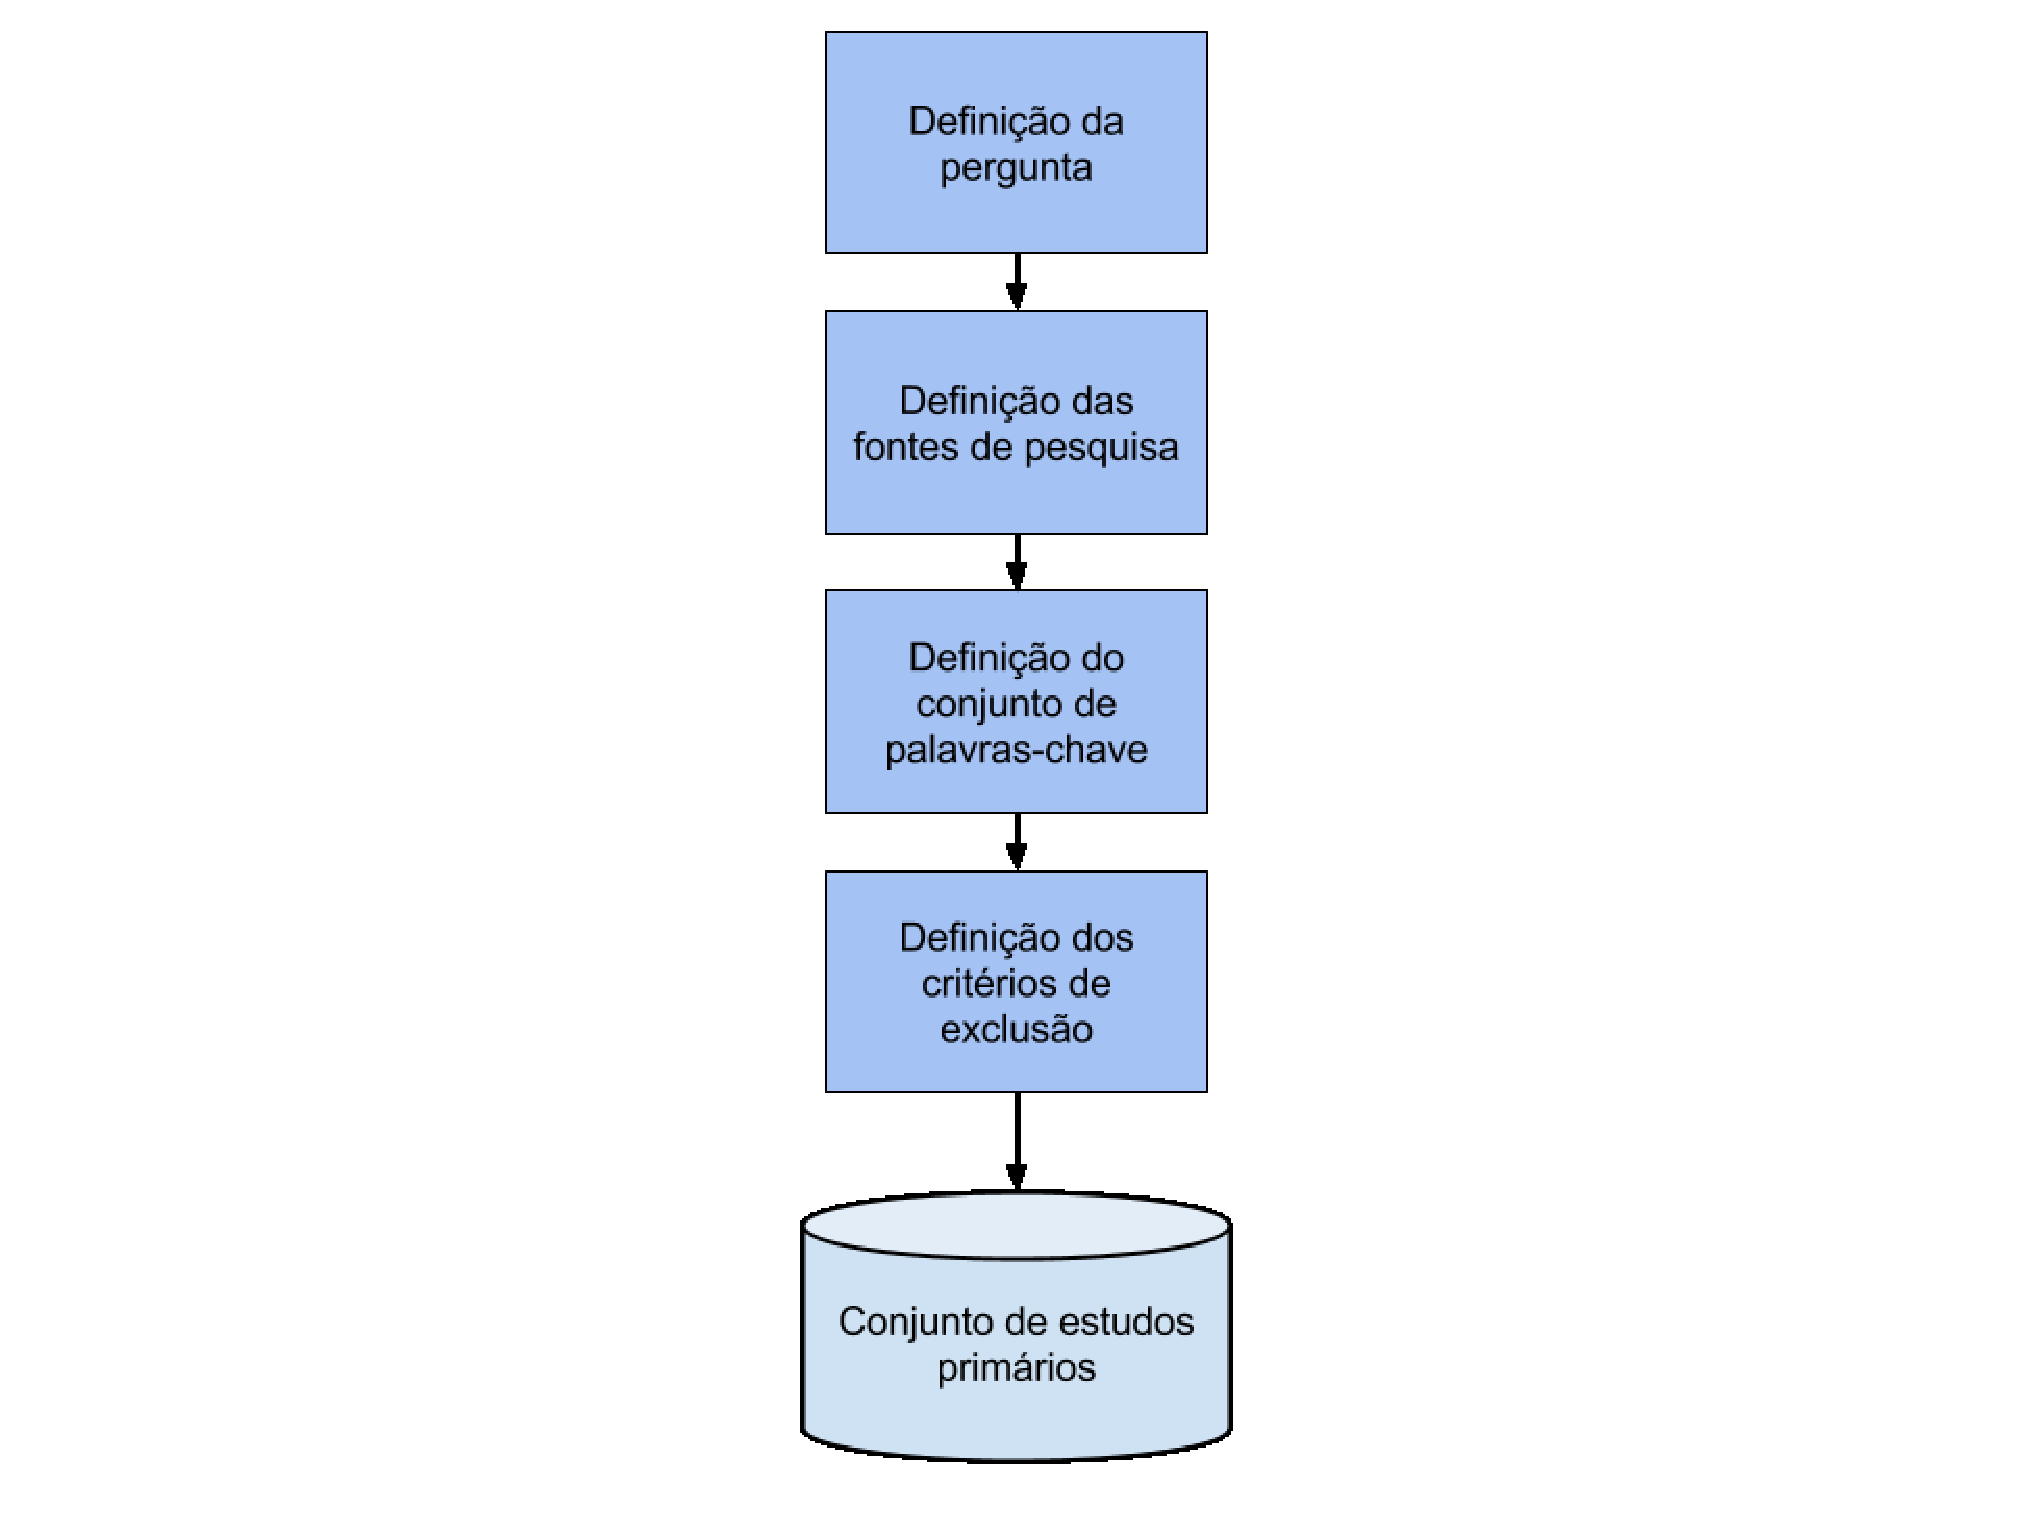
\includegraphics[scale=0.35]{capitulos/literatura/metodologia.eps}
	\caption{Diagrama que ilustra a metodologia de pesquisa utilizada para encontrar artigos científicos sobre adoção ágil}
	\label{fig:metodologia}
\end{figure}

Como dito inicialmente, o método utilizado foi baseado no proposto por Bárbara Kitchenham em \cite{Barbara04}. A necessidade desta adaptação se deu por um conjunto de restrições de tempo, nível de detalhe necessário e contingente disponível.

\subsubsection{Definição da pergunta}

O primeiro passo foi definir a questão a ser respondida ao final da pesquisa: ``\textit{Quais as principais lições aprendidas com a adoção de metodologias ágeis por parte de empresas de desenvolvimento de software na atualidade?}".

\subsubsection{Bases de dados relevantes}

Após a definição da pergunta a ser respondida, o próximo passo foi definir as fontes de informação mais confiáveis e relevantes para o tema (Tabela \ref{tab:basesDeDados}).

\begin{table}[H]
	\centering
	\begin{tabular}{| l | r |} \hline \textbf{Nome} & \textbf{Referência} \\ \hline
		CAPES & http://www.capes.gov.br/ \\ \hline
		ACM & http://www.acm.org/ \\ \hline
		IEEE & http://ieeexplore.ieee.org/ \\ \hline
		Google Scholar & http://scholar.google.com/ \\ \hline
		Springer Link & http://link.springer.com/ \\ \hline
	\end{tabular}
	\caption{Bases de dados consultadas na pesquisa}
	\label{tab:basesDeDados}
\end{table}

\nomenclature{CAPES}{Coordenação de Aperfeiçoamento de Pessoal de Nível Superior}%
\nomenclature{ACM}{Association for Computing Machinery}%
\nomenclature{IEEE}{Instituto de Engenheiros Eletricistas e Eletrônicos}%

\subsubsection{Palavras-chave}

Neste passo, foram definidas as palavras-chave (Tabela \ref{tab:palavrasChave}) buscadas nas bases de dados selecionadas.

\begin{table}[H]
	\centering
	\begin{tabular}{| l |} \hline \textbf{Palavras-chave} \\ \hline
		Agile Adoption \\ \hline
	\end{tabular}
	\caption{Conjunto de palavras-chave utilizadas na pesquisa}
	\label{tab:palavrasChave}
\end{table}

\subsubsection{Critérios de exclusão}

A base da literatura foi selecionada através do critério de exclusão de artigos. Como existem diversos materiais publicados na área de adoção ágil nas bases de dados selecionadas, foram encontrados cerca de 1000 artigos utilizando-se o conjunto de palavras-chave \textit{``Agile Adoption"}.

Porém, muitos dos dados coletados nesta pesquisa preliminar eram muito antigos, poderiam não fazer mais muito sentido nos dias atuais. Sendo assim, foi adicionado um segundo critério de exclusão: a data de publicação. Apenas materiais atuais (entre 2010 e 2013) seriam analisados. O contingente de trabalhos passou para, em média, 550 artigos.

Outro ponto importante a ser levado em consideração é a relevância do tema nos trabalhos restantes. O próximo filtro aplicado foi o de se encontrar as palavras-chave no título ou resumo. Com isso, o número de trabalhos reduziu bastante, para cerca de 50 artigos. Um ponto que vale a pena ser mencionado é que, nesta etapa do processo, caso o critério fosse levado extremamente à risca, bons materiais seriam eliminados. Este fator foi analisado na etapa posterior.

O último critério de exclusão utilizado nesta pesquisa foi uma análise qualitativa do material restante. Após uma revisão, artigo por artigo, 16 foram escolhidos, estando 2 deles fora do critério de exclusão anterior. A Tabela  \ref{tab:quantidadeDeMateriais} mostra com detalhes a quantidade de materiais selecionados em cada etapa.

\begin{table}[H]
	\centering
	\begin{tabular}{| c | l | r |} \hline \textbf{Critério de exclusão} & \textbf{Base de dados}  & \textbf{Quantidade} \\ \hline
		\multirow{4}{*}{-}
			& ACM & 106 \\ \cline{2-3}
			& CAPES & 51 \\ \cline{2-3}
			& Google Scholar & 849 \\ \cline{2-3}
			& IEEE & 30 \\ \cline{2-3}
			& Springer Link & 6 \\ \cline{2-3}
		\hline \hline
		\multirow{4}{*}{Artigos entre 2010 e 2013} 
			& ACM & 26 \\ \cline{2-3}
			& CAPES & 37 \\ \cline{2-3}
			& Google Scholar & 459 \\ \cline{2-3}
			& IEEE & 16 \\ \cline{2-3}
			& Springer Link & 5 \\ \cline{2-3}
		\hline \hline
		\multirow{4}{*}{Palavras-chave no título e/ou resumo} 
			& ACM & 1 \\ \cline{2-3}
			& CAPES & 2 \\ \cline{2-3}
			& Google Scholar & 38 \\ \cline{2-3}
			& IEEE & 14 \\ \cline{2-3}
			& Springer Link & 0* \\ \cline{2-3}
		\hline \hline
		\multirow{4}{*}{Análise crítica}
			& ACM & 0 \\ \cline{2-3}
			& CAPES & 0 \\ \cline{2-3}
			& Google Scholar & 4 \\ \cline{2-3}
			& IEEE & 10 \\ \cline{2-3}
			& Springer Link & 2 \\ \cline{2-3}
		\hline
	\end{tabular}
	\captionsetup{justification=centering}
	\caption{Quantidade de material encontrado em cada passo da pesquisa}
	\label{tab:quantidadeDeMateriais}
\end{table}

\subsection{Artigos selecionados}

O produto final desta revisão sistemática é um conjunto de trabalhos acadêmicos relevantes à pesquisa (Tabelas \ref{tab:artigosIEEE}, \ref{tab:artigosGoogle} e \ref{tab:artigosSpringer}).

\begin{table}[h]
	\centering
	\captionsetup{justification=centering,margin=1cm}
	\begin{tabularx}{\linewidth}{ | X | p{3cm} | } \hline \multicolumn{2}{|c|}{\textbf{Base de dados: IEEE}} \\ \hline
	\multicolumn{1}{|c|}{\textbf{Título do artigo}} & \multicolumn{1}{|c|}{\textbf{Referência}} \\ \hline
		Agile Adoption Experience: A Case Study in the U.A.E & \cite{Hajjdiab2011} \\ \hline
		Evolving to Agile: A story of agile adoption at a small SaaS company & \cite{Block2011} \\ \hline
		Factor Analysis: Investigating Important Aspects for Agile Adoption in Malaysia & \cite{Asnawi2012} \\ \hline
		Adobe Premiere Pro Scrum Adoption: How an agile approach enabled success in a hyper-competitive landscape & \cite{Adobe2012} \\ \hline
		Scaling Agile Methods to Regulated Environments: An Industry Case Study & \cite{Fitzgerald2013} \\ \hline
		The Maturation of Agile Software Development Principles and Practice: Observations on Successive Industrial Studies in 2010 and 2012 & \cite{Bustard2013} \\ \hline
		Have Agile Techniques been the Silver Bullet for Software Development at Microsoft? & \cite{Microsoft2013} \\ \hline
		The Agile Office: Experience Report from Cisco’s Unified Communications Business Unit & \cite{Cisco2011} \\ \hline
		The impact of agile principles and practices on large-scale software development projects A multiple-case study of two projects at Ericsson & \cite{Ericsson2013} \\ \hline
		Evaluating the Effect of Agile Methods on Software Defect Data and Defect Reporting Practices & \cite{Korhonen2010} \\ \hline
	\end{tabularx}
	\caption{Artigos científicos utilizados na pesquisa encontrados na base de dados IEEE}
	\label{tab:artigosIEEE}
\end{table}

\begin{table}[h]
	\centering
	\captionsetup{justification=centering,margin=1cm}
	\begin{tabularx}{\linewidth}{ | X | p{3cm} | } \hline \multicolumn{2}{|c|}{\textbf{Base de dados: Google Scholar}} \\ \hline
	\multicolumn{1}{|c|}{\textbf{Título do artigo}} & \multicolumn{1}{|c|}{\textbf{Referência}} \\ \hline
		DoD Agile Adoption: Necessary Considerations, Concerns, and Changes & \cite{Lapham2012} \\ \hline
		Software Tools and Processes: A Key Factor in Successful Agile Adoption & \cite{Arikpo2011} \\ \hline
		Inclusion of e-Assist to increase Agile Adoption & \cite{Radha2012} \\ \hline
		Agile Adoption Story from NHN & \cite{Eunha2012} \\ \hline
	\end{tabularx}
	\caption{Artigos científicos utilizados na pesquisa encontrados na base de dados Google Scholar}
	\label{tab:artigosGoogle}
\end{table}

\begin{table}[h]
	\centering
	\captionsetup{justification=centering,margin=1cm}
	\begin{tabularx}{\linewidth}{ | X | p{3cm} | } \hline \multicolumn{2}{|c|}{\textbf{Base de dados: Springer Link}} \\ \hline
	\multicolumn{1}{|c|}{\textbf{Título do artigo}} & \multicolumn{1}{|c|}{\textbf{Referência}} \\ \hline
		The evolution of agile software development in Brazil: Education, research, and the state-of-the-practice & \cite{Claudia2013} \\ \hline
		Evaluating the impact of an agile transformation: a longitudinal case study in a distributed  & \cite{Nokia2013} \\ \hline
	\end{tabularx}
	\caption{Artigos científicos utilizados na pesquisa encontrados na base de dados Springer Link}
	\label{tab:artigosSpringer}
\end{table}

O artigo \cite{Hajjdiab2011} apresenta um estudo de caso relatando o processo de adoção de métodos ágeis em uma entidade do governo do Emirados Árabes Unidos. \cite{Block2011} conta a história de adoção ágil de uma pequena empresa especializada em SaaS. \cite{Asnawi2012} foca na identificação de importantes aspectos na adoção ágil de de empresas de desenvolvimento de software da Malásia. \cite{Adobe2012} descreve como o pensamento ágil tem ajudado o Premiere Pro a ter ganhos significativos de vendas, qualidade e sustentabilidade. O estudo \cite{Fitzgerald2013} identifica pontos de tensão em adoção ágil e os ilustra através de um detalhado caso em que uma abordagem ágil foi implementada com sucesso em um ambiente controlado. A proposta de \cite{Bustard2013} é descrever o resultado de uma pesquisa feita na indústria cujo foco é entender a maturidade do modelo ágil no norte da Irlanda. \cite{Microsoft2013} rastreia as mudanças de atitude e técnicas do processo de adoção ágil na Microsoft através de uma grande pesquisa longitudinal durante um período de seis anos. O artigo \cite{Cisco2011} relata uma experiência da Cisco ao estabelecer um escritório ágil, descrevendo seu background histórico, o modelo de governança, onde ele se encaixa na estrutura da organização, atividades primárias, desafios encontrados, etc. A proposta da pesquisa \cite{Ericsson2013} feita na Ericsson é contribuir com evidências empíricas do impacto do uso de princípios e práticas ágeis na indústria em projetos de larga-escala. O estudo \cite{Korhonen2010} analisa os dados de defeitos encontrados num projeto distribuído de uma empresa nos seus doze primeiros meses de transformação ágil. O trabalho \cite{Lapham2012} relata um caso de um processo adoção ágil feito no Departamento de Defesa dos Estados Unidos. O artigo \cite{Arikpo2011} tem como foco principal discutir as demandas de gerências de requisito, projeto e configuração, além de processos e ferramentas que facilitam o processo de adoção ágil. O estudo \cite{Radha2012} discute os riscos envolvidos se pessoas não-capacitadas são escolhidas para desenvolver utilizando ágil, bem como maneiras de mitigá-los. \cite{Eunha2012} mostra como começar o processo de transição para desenvolvimento ágil através de dicas, tutoriais orientando como mover times de desenvolvimento de cascata para ágil, análise de benefícios e de possíveis problemas. No artigo \cite{Claudia2013} é apresentada uma visão global da evolução do movimento ágil no Brasil, seus principais defensores na academia e na indústria, iniciativas educacionais e uma pesquisa que mostra o estado da arte da indústria de TI no Brasil. O paper \cite{Nokia2013} é baseado nos resultados de um estudo de caso que analisa o impacto que a introdução de práticas ágeis fez em uma grande companhia que faz parte da Nokia Siemens Networks.

\nomenclature{SaaS}{Software as a Service}%
\nomenclature{TI}{Tecnologia da Informação}%

\section{Relatos de experiência}

Como o objetivo desta pesquisa é descobrir as principais lições aprendidas por parte de empresas de desenvolvimento de software ao tentar adotar Ágil, as apresentações em conferências não poderiam ser ignoradas.

\subsection{Método de pesquisa}

Para a seleção de relatos de experiência foi feita uma pesquisa exploratória, método bem mais flexível se comparado à revisão sistemática. As fontes utilizadas nesta etapa foram as conferências de Engenharia de Software mais importantes do mundo, como: \textit{``Agile Conference",``Agile Brazil",``Agile Mumbai",``Agile Goa"}, etc.

Uma análise qualitativa foi efetuada em cada material encontrado, mantendo-se o critério de necessitar serem trabalhos recentes.

\subsection{Relatos selecionados}

A Tabela \ref{tab:relatosEncontrados} mostra algumas informações a respeito dos relatos de experiência selecionados para a pesquisa (título, conferência e ano em que foram apresentados).

\begin{table}[h]
	\centering
	\captionsetup{justification=centering,margin=1cm}
	\begin{tabular}{| c | c | m{8cm} | m{2.5cm} |} \hline \textbf{Ano} & \textbf{Conferência}  & \textbf{Título do trabalho} & \textbf{Referência} \\ \hline
		\multirow{1}{*}{2008}
			& Agile Mumbai & Value-Driven Agile Adoption & \cite{Ahmed2008} \\ \cline{2-4}
		\hline \hline
		\multirow{4}{*}{2012}
			& \multirow{1}{*}{Agile Conference}
				& An Agile Adoption and Transformation Survival Guide & \cite{Sahota2012} \\ \cline{2-4}
			& \multirow{2}{*}{Agile Brazil}
				& Abolições Aprendidas: agilidade fora do contexto ideal & \cite{Piegas2012} \\ \cline{3-4}
				&& Implantando a Cultura Ágil em Larga Escala & \cite{Parzinello2012} \\ \cline{2-4}
			& \multirow{1}{*}{Agile Goa}
				& Agile in IT services & \cite{Srinath2012} \\ \cline{2-4}
		\hline \hline
		\multirow{18}{*}{2013}
			& \multirow{4}{*}{Agile Conference}
				& Evolving to Agile: transforming a public sector organization & \cite{Karaj2013} \\ \cline{3-4}
				&& Lean Change: Enabling Agile Transformation through Lean Startup, Kanban, and Kotter & \cite{Hui2013} \\ \cline{2-4}
			& \multirow{12}{*}{Agile Brazil}
				& 4 atitudes para melhorar a agilidade de uma empresa. Na prática. & \cite{Valerio2013} \\ \cline{3-4}
				&& Desafios do Desenvolvimento Ágil para o Governo & \cite{Stefano2013} \\ \cline{3-4}
				&& Padrões e Antipadrões da Adoção da Agilidade em Governo & \cite{Rodrigues2013} \\ \cline{3-4}
				&& Agilidade das Trincheiras do Tribunal Superior de Trabalho & \cite{Vieira2013} \\ \cline{3-4}
				&& Agile Black Ops - Como infiltrar agile em ambiente hostil & \cite{Queiroz2013} \\ \cline{3-4}
				&& Adoção de práticas ágeis no desenvolvimento de software de missão crítica & \cite{Bastos2013} \\ \cline{3-4}
				&& A incrível História de uma Organização Pública que Acredita em Agilidade & \cite{Maciel2013} \\ \cline{2-4}
		\hline
	\end{tabular}
	\caption{Relatos de experiência utilizados na pesquisa encontrados na principais conferências relevantes}
	\label{tab:relatosEncontrados}
\end{table}

A apresentação\cite{Ahmed2008} demonstra um framework para auxiliar no processo de adoção ágil. O trabalho \cite{Sahota2012} cria um guia para não apenas se adotar ágil, mas sim transformar a sua organização, fazer com que ela de fato seja ágil. \cite{Piegas2012} lista dezessete lições aprendidas ao se adotar ágil fora do contexto ideal. O relato \cite{Parzinello2012} compartilha uma experiência sobre um processo de adesão ágil gradual em larga escala. O conteúdo de \cite{Srinath2012} é relacionado a desafios e lições aprendidas descobertas durante a utilização de Ágil em uma organização de serviços de TI. \cite{Karaj2013} detalha todo o processo de maturação e uso de metodologias ágeis em uma organização pública. A apresentação \cite{Hui2013} demonstra princípios de Lean Startup auxiliando no processo de transformação ágil. No relato de experiência \cite{Valerio2013} conta-se sobre algumas práticas e atitudes tomadas em uma equipe em formação, com o objetivo de alinhar e compartilhar o conhecimento entre todos, evitando as chamadas ilhas de conhecimento. \cite{Stefano2013} compartilha desafios enfrentados pela empresa Digitho Brasil ao adotar uma abordagem de desenvolvimento ágil para o governo. O trabalho \cite{Rodrigues2013} mostra o caso de adoção ágil do VisPublica (projeto sobre visualização de dados públicos). A palestra \cite{Vieira2013}, apresentada no Agile Brazil 2013 em Brasília-DF, relata sobre problemas e soluções encontradas pelo TST na implantação de métodos ágeis de desenvolvimento de software. \cite{Queiroz2013}, utilizando uma abordagem problema/solução/resultado, compartilha experiências sobre o uso de metodologias ágeis em ambientes hostis (não-ideais). A apresentação \cite{Bastos2013} demonstra o impacto causado por Ágil num projeto chamado Ecossistema de Urna, responsável pela automação de atividades e processos envolvendo a urna eletrônica no Brasil. \cite{Maciel2013} é um relato de experiência do SERPRO Recife sobre sua busca pela agilidade.

\nomenclature{TST}{Tribunal Superior do Trabalho}%